\chapter{Regularization: Preventing Overfitting}\label{ch:regularization}
\begin{center}\small\textit{A network with millions of weights can memorize your dataset -- and fail on the next photo. Regularization teaches it to generalize.}\end{center}

\noindent\fbox{\parbox{\dimexpr\linewidth-2\fboxsep-2\fboxrule}{%
\textbf{From zero: no regularization background assumed.} We start from memorization versus learning and build to weight decay, dropout, augmentation, and early stopping. Every formula is preceded by a picture; overfitting is defined on first use.}}
\vspace{0.3em}
\section*{Learning Outcomes}
After this chapter you will be able to:
\begin{enumerate}[label=(L\arabic*)]
    \item explain overfitting and the bias--variance tradeoff;
    \item write the $L_2$-regularized loss and compare $L_1$/$L_2$ and elastic net;
    \item explain how dropout, augmentation, and early stopping curb memorization;
    \item diagnose under- and over-regularization from train/val curves.
\end{enumerate}

\section{Intuition: Memorization vs Learning}
A 10M-parameter network can fit 50k CIFAR images perfectly, even with random labels -- it merely memorizes. What we want is \textbf{generalization}: low error on unseen data. The gap between train and test error is \textbf{overfitting}. Regularization injects constraints or noise so the network cannot memorize quirks.

Think of fitting points with a polynomial: degree-15 fits noise wiggles; degree-3 captures the trend. The bias--variance tradeoff formalizes this: simple models underfit (high bias), complex models overfit (high variance), regularized models balance.

\section{Weight Decay (\texorpdfstring{$L_2$}{L2} Regularization)}
Penalize large weights:
\begin{equation}
\mathcal{L}_{\text{reg}}=\mathcal{L}_{\text{data}}+\lambda\|\mathbf{w}\|_2^2=\mathcal{L}_{\text{data}}+\lambda\sum_i w_i^2
\end{equation}
Gradient step becomes
\begin{equation}
\mathbf{w}\leftarrow(1-2\eta\lambda)\mathbf{w}-\eta\nabla\mathcal{L}_{\text{data}}
\end{equation}
so weights decay toward zero each step (hence ``weight decay''). Large $\lambda$ forces small weights $\to$ smoother functions $\to$ less overfitting. $L_1$ ($\lambda\sum|w_i|$) instead promotes sparsity.

In AdamW (Loshchilov \& Hutter, 2019), decay is decoupled: $\mathbf{w}\leftarrow\mathbf{w}-\eta(\hat{\mathbf{m}}/(\sqrt{\hat{\mathbf{v}}}+\epsilon)+\lambda\mathbf{w})$, fixing Adam's improper $L_2$ interaction with adaptive scaling.

\section{Dropout}
During training, randomly zero each hidden unit with probability $p$ (typically $0.2$--$0.5$):
\begin{equation}
\tilde{\mathbf{a}}^{(l)}=\mathbf{m}\odot\mathbf{a}^{(l)},\quad m_j\sim\text{Bernoulli}(1-p)
\end{equation}
At test time, scale by $(1-p)$ (or use inverted dropout: divide by $(1-p)$ during train, no scaling at test). Dropout trains an implicit ensemble of $2^H$ sub-networks sharing weights; at inference we average them. It breaks co-adaptation: no neuron can rely on a specific partner being present.

\begin{center}
\begin{tikzpicture}[font=\scriptsize, >=Stealth, scale=0.92]
  % Without dropout
  \begin{scope}
    \foreach \i in {1,2,3} \node[circle, draw, fill=blue!15, minimum size=0.7cm] (a\i) at (0,-\i*0.9) {};
    \foreach \i in {1,2,3} \node[circle, draw, fill=green!15, minimum size=0.7cm] (b\i) at (1.8,-\i*0.9) {};
    \foreach \i in {1,2} \foreach \j in {1,2,3} \draw[->, gray!60, thin] (a\i) -- (b\j);
    \node[above, font=\tiny] at (0.9,-0.3) {Full network};
  \end{scope}
  % With dropout
  \begin{scope}[shift={(4.5,0)}]
    \foreach \i in {1,2,3} \node[circle, draw, fill=blue!15, minimum size=0.7cm] (c\i) at (0,-\i*0.9) {};
    \node[circle, draw, fill=gray!20, minimum size=0.7cm, opacity=0.35] (d1) at (1.8,-0.9) {$\times$};
    \node[circle, draw, fill=green!15, minimum size=0.7cm] (d2) at (1.8,-1.8) {};
    \node[circle, draw, fill=gray!20, minimum size=0.7cm, opacity=0.35] (d3) at (1.8,-2.7) {$\times$};
    \foreach \i in {1,2,3} \draw[->, orange!70!black, thin] (c\i) -- (d2);
    \draw[->, gray!30, dashed] (c1) -- (d1); \draw[->, gray!30, dashed] (c2) -- (d3);
    \node[above, font=\tiny, text=orange!70!black] at (0.9,-0.3) {Dropout ($p=0.5$)};
  \end{scope}
  % Ensemble
  \begin{scope}[shift={(8.5,0)}]
    \node[draw, fill=violet!10, rounded corners, minimum width=2.2cm, minimum height=2.2cm, align=center, font=\tiny] at (0,-1.8) {Implicit ensemble\\of $2^{H}$ sub-nets\\{\scriptsize avg at test}};
    \draw[->, thick, violet!60!black] (6.3,-1.8) -- (7.4,-1.8);
  \end{scope}
\end{tikzpicture}
\end{center}

\section{Data Augmentation \& Early Stopping}
\textbf{Augmentation} expands data by label-preserving transforms: for images, random crop, flip, rotation, color jitter, Cutout/Mixup; for text, synonym replace, back-translation. More diverse data $\to$ less memorization.

\textbf{Early stopping}: monitor validation loss; stop when it rises for $P$ epochs (patience). This is implicit $L_2$ control -- fewer steps $\to$ weights stay nearer initialization (small norm). Combined with checkpointing the best model, it is the simplest regularizer that almost always helps.

\begin{center}
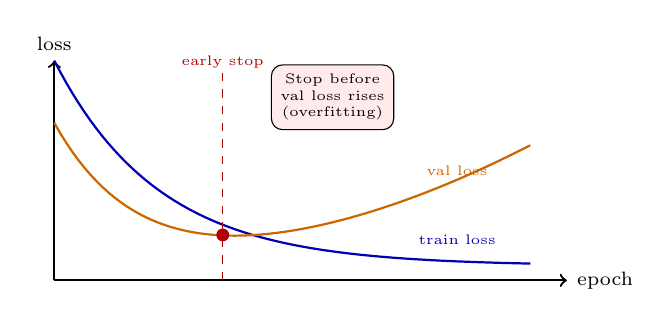
\begin{tikzpicture}[font=\scriptsize, scale=0.93]
  \draw[->, thick] (0,0) -- (7,0) node[right] {epoch};
  \draw[->, thick] (0,0) -- (0,3) node[above] {loss};
  \draw[thick, blue!70!black, domain=0:6.5, samples=80] plot (\x, {2.8*exp(-0.7*\x)+0.2});
  \node[blue!70!black, font=\tiny] at (5.5,0.55) {train loss};
  \draw[thick, orange!80!black, domain=0:6.5, samples=80] plot (\x, {2.0*exp(-0.9*\x)+0.15+0.04*\x*\x});
  \node[orange!80!black, font=\tiny] at (5.5,1.5) {val loss};
  \draw[dashed, red!70!black] (2.3,0) -- (2.3,2.85) node[above, fill=white, inner sep=1pt, font=\tiny] {early stop};
  \fill[red!70!black] (2.3,0.62) circle (2.5pt);
  \node[draw, fill=red!8, rounded corners, font=\tiny, align=center] at (3.8,2.5) {Stop before\\val loss rises\\(overfitting)};
\end{tikzpicture}
\end{center}

\section{Putting It Together}
\begin{example}[PyTorch Regularization Cocktail]
\begin{lstlisting}[language=Python]
import torch.nn as nn
class RegularizedMLP(nn.Module):
    def __init__(self, p_drop=0.5, wd=1e-4):
        super().__init__()
        self.net = nn.Sequential(
            nn.Linear(784, 512), nn.ReLU(), nn.Dropout(p_drop),
            nn.Linear(512, 256), nn.ReLU(), nn.Dropout(p_drop),
            nn.Linear(256, 10)
        )
        self.wd = wd
    def forward(self, x): return self.net(x.view(x.size(0),-1))

model = RegularizedMLP(p_drop=0.3)
opt = torch.optim.AdamW(model.parameters(), lr=1e-3, weight_decay=1e-4)  # decoupled wd
aug = nn.Sequential()  # placeholder: use torchvision.transforms
# Training loop with early stopping
best_val, patience, wait = float('inf'), 5, 0
for epoch in range(100):
    model.train()
    for x,y in train_loader:  # x augmented: RandomCrop, HorizontalFlip
        opt.zero_grad()
        loss = nn.CrossEntropyLoss()(model(x), y)
        loss.backward(); opt.step()
    # validation
    model.eval()
    val_loss = sum(nn.CrossEntropyLoss()(model(x),y).item() for x,y in val_loader)/len(val_loader)
    if val_loss < best_val: best_val=val_loss; wait=0; torch.save(model.state_dict(),"best.pt")
    else: wait+=1
    if wait>=patience: print(f"Early stop at {epoch}"); break
model.load_state_dict(torch.load("best.pt"))
\end{lstlisting}
\end{example}

A complementary technique is \textbf{label smoothing}: replace one-hot $y_k$ with $(1-\epsilon)y_k+\epsilon/K$, discouraging overconfident logits.

\section{Regularization Spectrum}
\begin{center}
\begin{tikzpicture}[font=\scriptsize, >=Stealth]
  \node[draw, fill=red!10, rounded corners, minimum width=2.0cm, minimum height=0.8cm, align=center] (a) at (0,0) {Large weights\\overfit};
  \node[draw, fill=orange!12, rounded corners, minimum width=2.0cm, minimum height=0.8cm] (b) at (3.5,0) {\small Weight decay};
  \node[draw, fill=green!12, rounded corners, minimum width=2.0cm, minimum height=0.8cm] (c) at (7,0) {\small Dropout};
  \node[draw, fill=blue!12, rounded corners, minimum width=2.0cm, minimum height=0.8cm] (d) at (10.5,0) {\small Augment + Early stop};
  \draw[->, thick, gray!60!black] (a) -- (b); \draw[->, thick, gray!60!black] (b) -- (c); \draw[->, thick, gray!60!black] (c) -- (d);
  \node[below=0.4cm of b, font=\tiny, align=center, text=gray!60!black] {shrinks\\weights};
  \node[below=0.4cm of c, font=\tiny, align=center, text=gray!60!black] {breaks\\co-adapt};
  \node[below=0.4cm of d, font=\tiny, align=center, text=gray!60!black] {more data\\less steps};
\end{tikzpicture}
\end{center}

\section{Bias--Variance Tradeoff Formalized}
For squared loss, expected test error decomposes:
$\mathbb{E}[(y-\hat f(x))^2]=\text{Bias}^2+\text{Var}+\sigma^2_{\text{noise}}$.
Capacity $\uparrow$ lowers bias but raises variance. Regularization traces a
U-curve: too little $\to$ overfit (high var), too much $\to$ underfit (high
bias). Validation curves (train vs val loss versus $\lambda$ or $p$) locate the
sweet spot. Cross-validation refines this when data are scarce.

\section{Weight Decay vs \texorpdfstring{$L_1$}{L1} and Elastic Net}
$L_2$ shrinks weights smoothly; $L_1$ ($\lambda\sum|w_i|$) yields sparsity via
soft-thresholding -- useful for feature selection. Elastic net mixes both:
$\lambda_1\|\mathbf{w}\|_1+\lambda_2\|\mathbf{w}\|_2^2$. In deep nets, $L_2$ is
dominant because we rarely want exact zeros in dense layers, but $L_1$ appears
in pruning and compressed sensing. Decoupled AdamW correctly separates decay
from gradient-based adaptivity, fixing the original Adam+$L_2$ bug.

\section{Dropout Variants and Analysis}
Standard dropout drops units; \textbf{DropConnect} drops weights, \textbf{Spatial
Dropout} drops whole feature maps (better for CNNs where neighbours correlate),
\textbf{Cutout/RandomErasing} drops image patches. At test time, Monte Carlo
dropout (keep dropout on, average many forwards) estimates uncertainty -- a
cheap Bayesian approximation (Gal \& Ghahramani, 2016). Inverted dropout's
scaling by $1/(1-p)$ during training keeps expected activation magnitude
constant, so no test-time rescaling is needed.

\section{Augmentation Zoo and Mixup}
Beyond crop/flip, modern augmentation includes: color jitter, Gaussian blur,
Mixup ($\tilde{\mathbf{x}}=\lambda\mathbf{x}_i+(1-\lambda)\mathbf{x}_j$,
$\tilde y$ mixed similarly -- encourages linear behaviour between examples),
CutMix (paste patches), and AutoAugment (learned policies). For NLP, back-
translation and EDA (random insert/delete/swap) help. Strong augmentation can
replace substantial labeled data -- a key reason ImageNet models train on
``infinite'' augmented streams rather than 1.2M fixed images.

\section{Common Pitfalls}
Applying dropout at test time without scaling ruins predictions -- use
\texttt{model.eval()} in PyTorch to disable it. Setting $\lambda$ too high
underfits; too low does nothing -- sweep $\lambda$ on a log scale and watch
the train--val gap. Augmentation that is too strong (e.g., 90-degree rotation
on digit 6$\to$9) changes labels and hurts. Validate augmentation by visual
inspection.

\section{Further Reading}
Srivastava et al. (2014) on dropout; Zhang et al. (2017) ``Understanding deep
learning requires rethinking generalization'' shows memorization power. For
augmentation, see Cubuk et al. AutoAugment and Zhang et al. Mixup. Early
stopping theory is in Yao et al. (2007) -- $L_2$ equivalence.

\section{Chapter Summary}
Capacity without constraint memorizes. $L_2$ shrinks weights; dropout trains an
ensemble of sub-nets; augmentation enlarges data; early stopping limits steps.
Together they close the train--val gap. AdamW decouples decay correctly; Mixup
and label smoothing further curb overconfidence. Regularization is not optional
at scale -- it is what makes generalization possible.

\smallskip
\noindent\textit{Key takeaways:} (1) $\mathcal{L}+\lambda\|\mathbf{w}\|^2$
decays weights; (2) dropout $p=0.2$--$0.5$ breaks co-adaptation;
(3) augmentation is free data; (4) early stopping $\approx L_2$;
(5) AdamW $>$ Adam+$L_2$ for adaptive methods.

\paragraph{Debugging regularization.} If train loss is high, regularization is too strong—reduce $\lambda$ or $p$. If val loss diverges early, increase augmentation. Plot weight histograms: $L_2$ keeps them Gaussian, dropout keeps them sparse.

\begin{example}[Dropout expectation] For input $x=2$ and mask $m\sim\text{Bernoulli}(0.5)$, training output $y=m\cdot x/0.5$ has $\mathbb{E}[y]=2$. Inverted dropout scales at train time, so test time needs no scaling. This preserves $\mathbb{E}[y_{\text{train}}]=\mathbb{E}[y_{\text{test}}]$.
\end{example}
\begin{remark}[Label smoothing] Replacing hard label $1$ with $0.9$ and $0$ with $0.1/(K-1)$ prevents overconfident logits, reducing $\|\mathbf{z}\|_2$ and improving calibration.
\end{remark}

\section{Exercises}
\begin{exercise} Show that $L_2$-regularized linear regression has closed form $\mathbf{w}= (X^{\top}X+\lambda I)^{-1}X^{\top}\mathbf{y}$. What happens as $\lambda\to\infty$?\end{exercise}
\begin{exercise} Dropout with $p=0.5$ on a layer of 1000 units: how many distinct sub-networks? Why is the test-time scaling by $0.5$ needed for expectation matching?\end{exercise}
\begin{exercise} Implement data augmentation for CIFAR-10: random crop + horizontal flip. Train a small CNN with and without augmentation; report train/test gap.\end{exercise}
\begin{exercise} Early stopping as regularization: sketch why stopping after $T$ SGD steps is similar to $L_2$ with $\lambda\propto1/T$. Hint: gradient flow path length.\end{exercise}
\begin{exercise} Compare Adam vs AdamW on a 4-layer MLP with $\lambda=10^{-2}$. Why does AdamW generalize better? Inspect effective weight-decay magnitude.\end{exercise}
% End of Chapter
